\chapter{Cost Model Spreadsheets}\label{app:B_cost_model_spreadsheets}

\section{Static NPV Model}\label{app:B_static_model}
The static model described in Section \ref{ch4:cm_concept} was implemented in Microsoft Excel as a single worksheet for cost analysis. Figures \ref{fig:static_model_sheet1} and \ref{fig:static_model_sheet2} show the model when flow rate is pre-defined and capacity depends on the input temperature of the produced brine. Not shown is the supporting look-up table for the EIA STEO-based electricity price forecast (Figure \ref{fig:electricity_pricing}).
\vfill
\pagebreak

\begin{figure}[H]
\centering
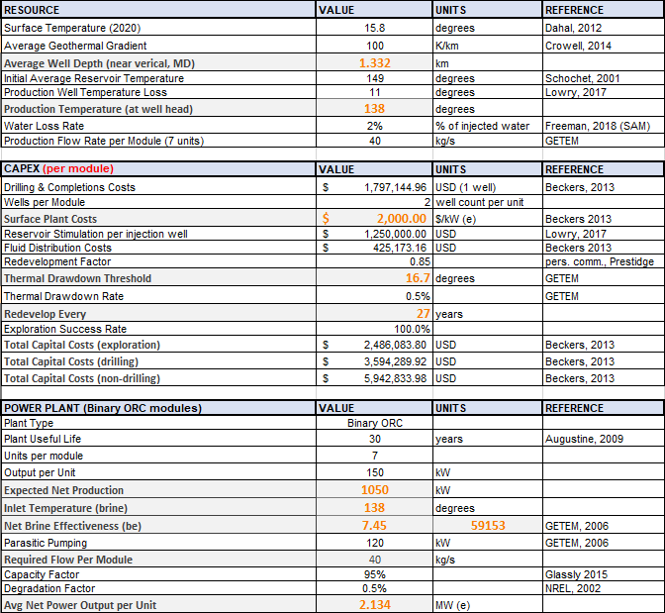
\includegraphics[width=\textwidth]{templates/images/Figure-Static_Model_SheetA.png}
\caption[Static cost model worksheet (part 1)]{First part of static NPV cost model for the geothermal expansion project.}
\label{fig:static_model_sheet1}
\end{figure}

\begin{figure}[H]
\centering
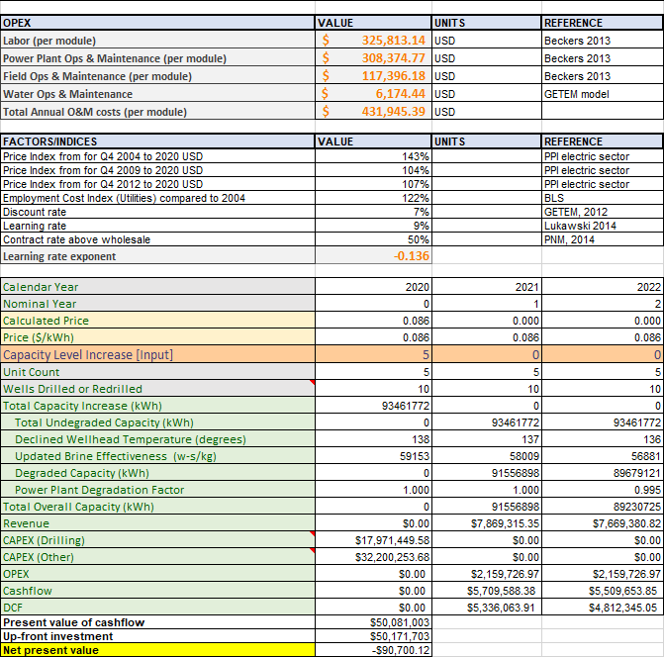
\includegraphics[width=\textwidth]{templates/images/Figure-Static_Model_SheetB.png}
\caption[Static cost model worksheet (part 2)]{Second part of static NPV cost model for the geothermal expansion project. The yearly breakdown of cost and revenue only extends out to year 2 for visualization purposes but continues to year 30 in the actual spreadsheet.}
\label{fig:static_model_sheet2}
\end{figure}
\pagebreak
\section{Probabilistic NPV Models}\label{app:B_flex_models}
The probabilistic NPV model was implemented as an extension of the static NPV model in Excel, with variable look-ups using the PDFs described in Section \ref{ch4:pdfs}. Flexible design options described in Section \ref{ch4:flex_design_options} were implemented as decision rules in the cash flow analysis. Figures \ref{fig:probabilistic_model_sheet1} and \ref{fig:probabilistic_model_sheet2} illustrate the spreadsheet for the Full Flexibility case (see Section \ref{ch4:flex_reduce_case}). The results histogram, target curve, and summary statistics were generated using a 2000-row data table tied to the NPV calculation cell (not shown).
\vfill
\pagebreak

\begin{figure}[H]
\centering
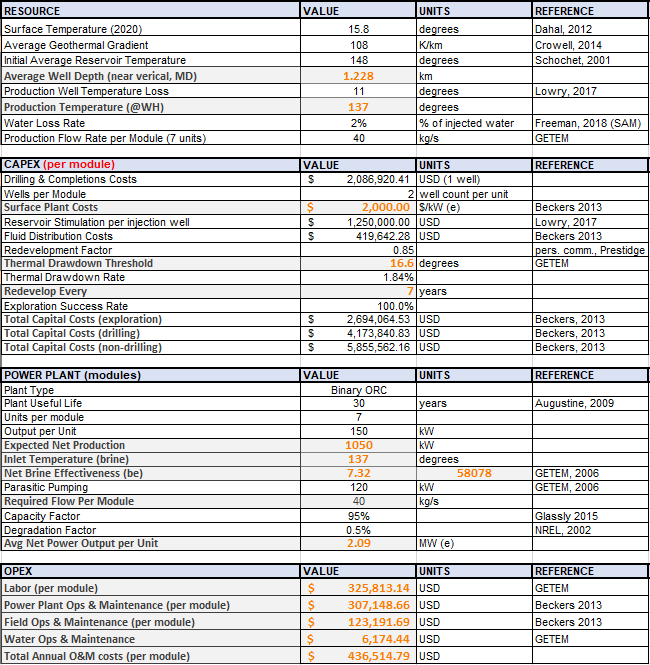
\includegraphics[width=\textwidth]{templates/images/Figure-Flexible_Model_SheetA.png}
\caption[Probabilistic cost model worksheet (part 1)]{First part of probabilistic NPV cost model for the geothermal expansion project. PDF look-ups were implemented for Average Geothermal Gradient, Initial Average Reservoir Temperature, Drilling \& Completions Costs, Thermal Drawdown Rate, and Price Forecast.}
\label{fig:probabilistic_model_sheet1}
\end{figure}

\begin{figure}[H]
\centering
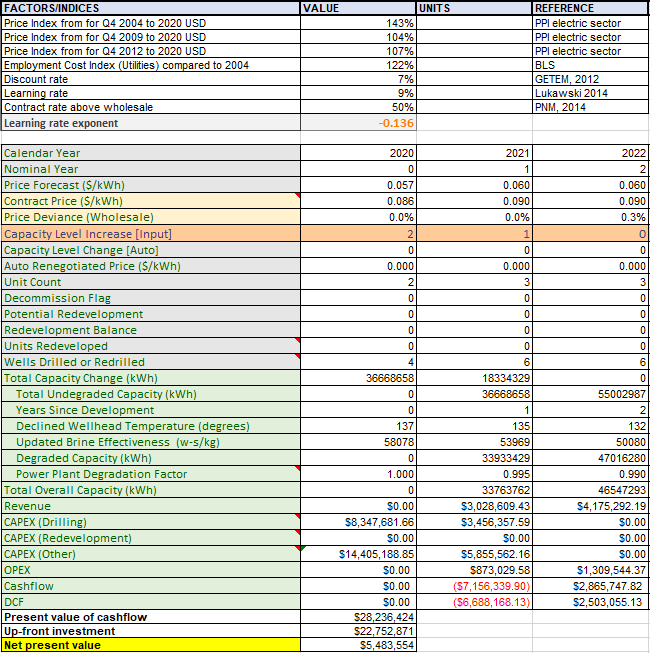
\includegraphics[width=\textwidth]{templates/images/Figure-Flexible_Model_SheetB.png}
\caption[Probabilistic cost model worksheet (part 2)]{Second part of probabilistic NPV cost model for the geothermal expansion project. PDF look-ups were implemented for Average Geothermal Gradient, Initial Average Reservoir Temperature, Drilling \& Completions Costs, Thermal Drawdown Rate, and Price Forecast. Decision rules are implemented in the annual cash flow section. The yearly breakdown of cost and revenue only extends out to year 2 for visualization purposes but continues to year 30 in the actual spreadsheet.}
\label{fig:probabilistic_model_sheet2}
\end{figure}